\chapter{Análise Bibliográfica sobre Simulação Multiagente e Fenômenos Sociais, por Jorge Fernandes\label{chap:bibliometria:jhcf}}

\section{Planejamento do estudo}
O planejamento o  desenho do estudo deve descrever as motivações, questões de interesse, escopo, limitações e objetivos do trabalho.

O planejamento do estudo deve motivar o tema escolhido e o interesse do autor.

No caso do meu trabalho, as perguntas que o nortearam foram:
\begin{itemize}
    \item Qual a base de conhecimentos científicos produzida em torno do tema simulação multiagente voltada à compreensão de fenômenos sociais, com ênfase em métodos experimentais? 
    \item Como a simulação multiagente tem sido usada para compreender fenômenos sociais, com ênfase em métodos experimentais? 
    \item Quais os principais termos e conceitos ligados à frente de pesquisa no tema simulação multiagente de fenômenos sociais, com ênfase em métodos experimentais? 
    \item Qual a estrutura social da comunidade, se é que existe, que pesquisa sobre o tema simulação multiagente de fenômenos sociais, com ênfase em métodos experimentais?
\end{itemize}

\subsection{O que já existe de pesquisa bibliométrica sobre esse tema?}

\cite{gore_classifying_2016} fizeram uma pesquisa que visava aprofundar a questão da simulação multiagente em relação à computação experimental.

A pesquisa é base para um posterior aprofundamento no campo da Cientometria, como fez \cite{chavalarias_whats_2017}.

\subsection{Uso do Bibliometrix e Biblioshiny}
Serão usadas a ferramenta e o \textit{workflow} proposto pelos autores do pacote Bibliometrix, conforme indica a figura ~\ref{fig:bibliometrix:workflow}.

\subsection{Limitações} O exercício relatado foi feito em uma semana, envolvendo entre 5 a 10 horas de trabalho de cada autor.

Outros aspectos a reforçar:
\begin{itemize}
   
\item Deve-se fazer buscas na base de dados WoS ou SCOPUS;
\item é obrigatório declarar um conjunto de perguntas de pesquisa.
\item é preciso declarar o objetivo da pesquisa, que no caso da aqui relatada foi exercitar inicialmente, e relatar, o uso da técnica de análise bibliométrica, para fins didáticos.
\end{itemize}


\section{Coleta de dados\label{MASSA:coleta}}

A coleta de dados feita usando o WoS no dia 03 de agosto de 2021, acessado por meio do Portal de Periódicos da CAPES.

Foram feitas buscas nas coleções \textbf{Science  Citation  Index  Expanded (SCI -EXPANDED)} e \textbf{Social  Sciences  Citation  Index (SSCI)}, que contém registros relativos a vários campos do conhecimento, no qual o SCI-EXPANDED foca mais na área das ciências exatas e naturais, enquanto que o SSCI indexa artigos da área das ciências sociais. Observe que os artigos nessas duas coleções são indexados desde 1945. 

Foi usada a \query\  de busca ilustrada nas linhas 1 a 9 da listagem \ref{query20210803-2}.

\lstinputlisting[numbers=left,basicstyle=\normalsize\ttfamily,caption={\query\  de busca sobre simulação multiagente de fenômenos socials, com ênfase em métodos experimentais.},label=query20210803-2]
{experiments/jhcf/PesqBibliogr/SimulacaoMultiagente/WoS-20210803/classico-mais-citacoes/query.txt}

\subsection{Explicação para os termos de busca usados\label{MASSA:query}}

A busca consistiu de quatro cláusulas disjuntivas, unidas por uma conjunção \textit{and}, aplicadas à busca por tópico (O termo de busca pode aparecer no Título, no Abstract, na Author Keywords, ou nas Keywords Plus da referência)

Os termos \texttt{experimental}, \texttt{numeric*}, \texttt{statist*}, \texttt{hypothes*}, 
\texttt{empiric*}
e \texttt{inferen} (linhas 1 e 2 da query) foram usados na primeira cláusula da \query\  para recuperar artigos que tenham em seu título, palavras-chave e resumo, termos relacionados a métodos experimentais,
métodos numéricos,
métodos estatísticos,
teste de hipóteses,
métodos empíricos e métodos inferenciais.

O termo / cláusula  \texttt{simul*}, na linha 4, foi usado em conjunção com os demais para recuperar apenas trabalhos que explicitem o uso da simulação.
Foi usado um único termo devido à forte adesão ao termo simulação por parte dos pesquisadores que usam simulação. Não existem outros sinônimos frequentes para esse uso.

A cláusula nas linhas 6 e 7 faz união entre o uso dos termos \texttt{agent} e \texttt{multiagent}, \texttt{multi-agent},e  também \texttt{multi and agent}, para cobrir as variadas formas de escrita do conceito.

A $4^{a}$ cláusula, linha 9,  usou os termos \texttt{social} e \texttt{society} para recuperar artigos que tratem de temas ligados à sociedade.
Os termos \texttt{group} e \texttt{behavi*} visam recuperar estudos que tratam de questões comportamentais e grupais.

Os 8.115 registros obtidos encontram-se no github do projeto, em \url{https://github.com/jhcf/Comput-Experim-20212/experiments/jhcf/PesqBibliogr/SimulacaoMultiagente/ WoS-20210803/classico-mais-citacoes/8115recs.txt}. 

Foram utilizadas as opções \textit{Exportar registros para arquivo de texto sem formatação} e \textit{export full record / Gravar Conteúdo: Seleção personalizada, com todos os 29 campos disponíveis, inclusive referências citadas} no WoS, para que as citações também fosse usadas em análises da citações (estrutura intelectual do conhecimento). Os 8115 registros foram recuperados em nove blocos de até 1.000 registros por vez (1-1000, 1001-2000, 2001-3000, ..., 8001-8115).

\section{Análise dos dados}

\subsection{Filtragem de registros}
Antes da análise, é possível aplicar filtros sobre os registros obtidos.

Foi aplicado um filtro ao \dataset\   inicial, com 8.115 registros, que continham pŕevias de artigos, artigos de conferência, capítulos de livro etc. Foram mantidos apenas os registros de artigos publicados em revistas científicas\footnote{A suposição é que que o conhecimento de maior qualidade sobre o tema está nas publicações em revistas.}. Após a aplicação desse filtro, 5.787 registros foram mantidos no \dataset, que será doravante chamado MultiAgentSimulationSociety/Artigos, ou MASSA@jhcf.

\subsection{Análise descritiva do \dataset\   MASSA@jhcf}

A análise bibliométrica descritiva faz uma descrição inicial do \dataset\  . Para explicação detalhada de como são calculadas as diversas taxas geradas pelo Bibliometrix veja a documentação do \textit{package} a partir da página \url{https://cran.r-project.org/web/packages/bibliometrix/index.html}. A análise bibliométrica descritiva é gerada pela função \texttt{biblioAnalysis}.

As informações mais gerais sobre o \dataset\   MASSA@jhcf são as seguintes:
\begin{description}
    \item [\textit{Timespan}] Os artigos que atenderam aos critérios de busca e filtragem foram publicados a partir de 1990, até 2021. Ou seja, não foram encontrados registros entre 1945 e 1989.
    \item [\textit{Sources (Journals, Books, etc)}] São 2.319 fontes de informação que publicaram os documentos recuperados no \dataset\   MASSA@jhcf. Ou seja, em média, cada \textit{scientific journal} publicou $5.787/2.319=2,5$ artigos. \footnote{Note que a média, enquanto medida de tendência central, pode não ser a que melhor reflete a tendência a quantidade de artigos publicados por revista.}
    \item [\textit{Average years from publication}] A média do tempo de publicação dos artigos no \dataset\   MASSA@jhcf é de 7,36 anos.
    \item [\textit{Average citations per documents}] Cada artigo no \dataset\   MASSA@jhcf foi citado, em média 20,7 vezes\footnote{Note que a média, enquanto medida de tendência central, pode não ser a que melhor reflete a tendência de  citações a artigos.}.
    \item [\textit{Average citations per year per doc}] Após publicado, cada um dos 5.787 artigos do \dataset\   MASSA@jhcf  foi citado 2,262 vezes por ano, em média.
    \item [\textit{References}] O \dataset\   MASSA@jhcf contém 201.464 referências citadas (tags CR).
    \item [\textit{Keywords Plus (ID)}] 13.735 distintas palavras-chave do tipo Keywords Plus (ID)\footnote{\textit{KeyWords Plus} são ``termos de índice gerados automaticamente a partir dos títulos de artigos citados. Os termos do KeyWords Plus devem aparecer mais de uma vez na bibliografia e são ordenados de frases com várias palavras a termos únicos. O KeyWords Plus aumenta o número de resultados tradicional de palavras-chave ou títulos.'' Fonte: \url{https://images.webofknowledge.com/WOKRS410B4/help/pt_BR/WOS/hp_full_record.html}} foram encontradas no \dataset\   MASSA@jhcf. 
    \item [\textit{Author's Keywords (DE)}] 15.704 distintas palavras-chave indicadas pelos autores foram encontradas no \dataset\  .
    \item [\textit{Authors}] 19.410 distintos nomes de autores foram encontrados no \dataset\  \footnote{Um mesmo autor pode ter uma ou mais diferentes grafias no \dataset\  , e serão reconhecidos dois ou mais autores diferentes, embora de fato sejam apenas um. Isso significa que a quantidade de \textbf{nomes de autores} equivale à quantidade de \textbf{autores}. Adicionalmente, é possível que distintos autores sejam reconhecidos com o mesmo nome, isso é, que sejam homônimos. Ou seja, o \dataset\   em geral conterá erros de contagem na quantidade de autores reais.}.
    \item [\textit{Author Appearances}] Os 19.410 distintos (nomes de) autores foram encontrados 23.470 vezes, como autores de artigos.
    \item [\textit{Authors of single-authored documents}] Dentre os 19.410 distintos (nomes de) autores encontrados, 375 deles editaram artigos individualmente, isso é, sem co-autores.
    \item [\textit{Authors of multi-authored documents}] Dentre os 19.410 distintos (nomes de) autores encontrados, 19.035 deles editaram artigos com um ou mais co-autores"
    \item [\textit{Single-authored documents}] Dentre os 5.787 documentos presentes no \dataset\   MASSA, 409 foram escritos por um único autor, e os 5.378 restantes foram elaborados em co-autoria.
    \item [\textit{Documents per Author}] Dentre os 19.410 distintos (nomes de) autores, cada um publicou em média 0,298 artigos.
    \item [\textit{Authors per Document}] Cada um dos 5.787 documentos presentes no \dataset\   MASSA foi autorado com 3,35 autores em média ($19.410 / 5.787 = 3,35$).
    \item [\textit{Co-Authors per Documents}] As 23.470 aparições de (nomes de) autores (``Author Appearances''), sem distribuem, em média 4,06 vezes para os 5.787 documentos do \dataset\   MASSA@jhcf.
    \item [\textit{Collaboration Index}] Os 19.035 (nomes de) autores que editaram artigos com um ou mais co-autores, colaboraram em media 3,54 vezes para editar os 5.378 artigos elaborados em co-autoria, gerando, assim, um índice de colaboração 3,54. 
\end{description}

\subsection{Evolução da Produção Científica}

\begin{figure}
    \centering
    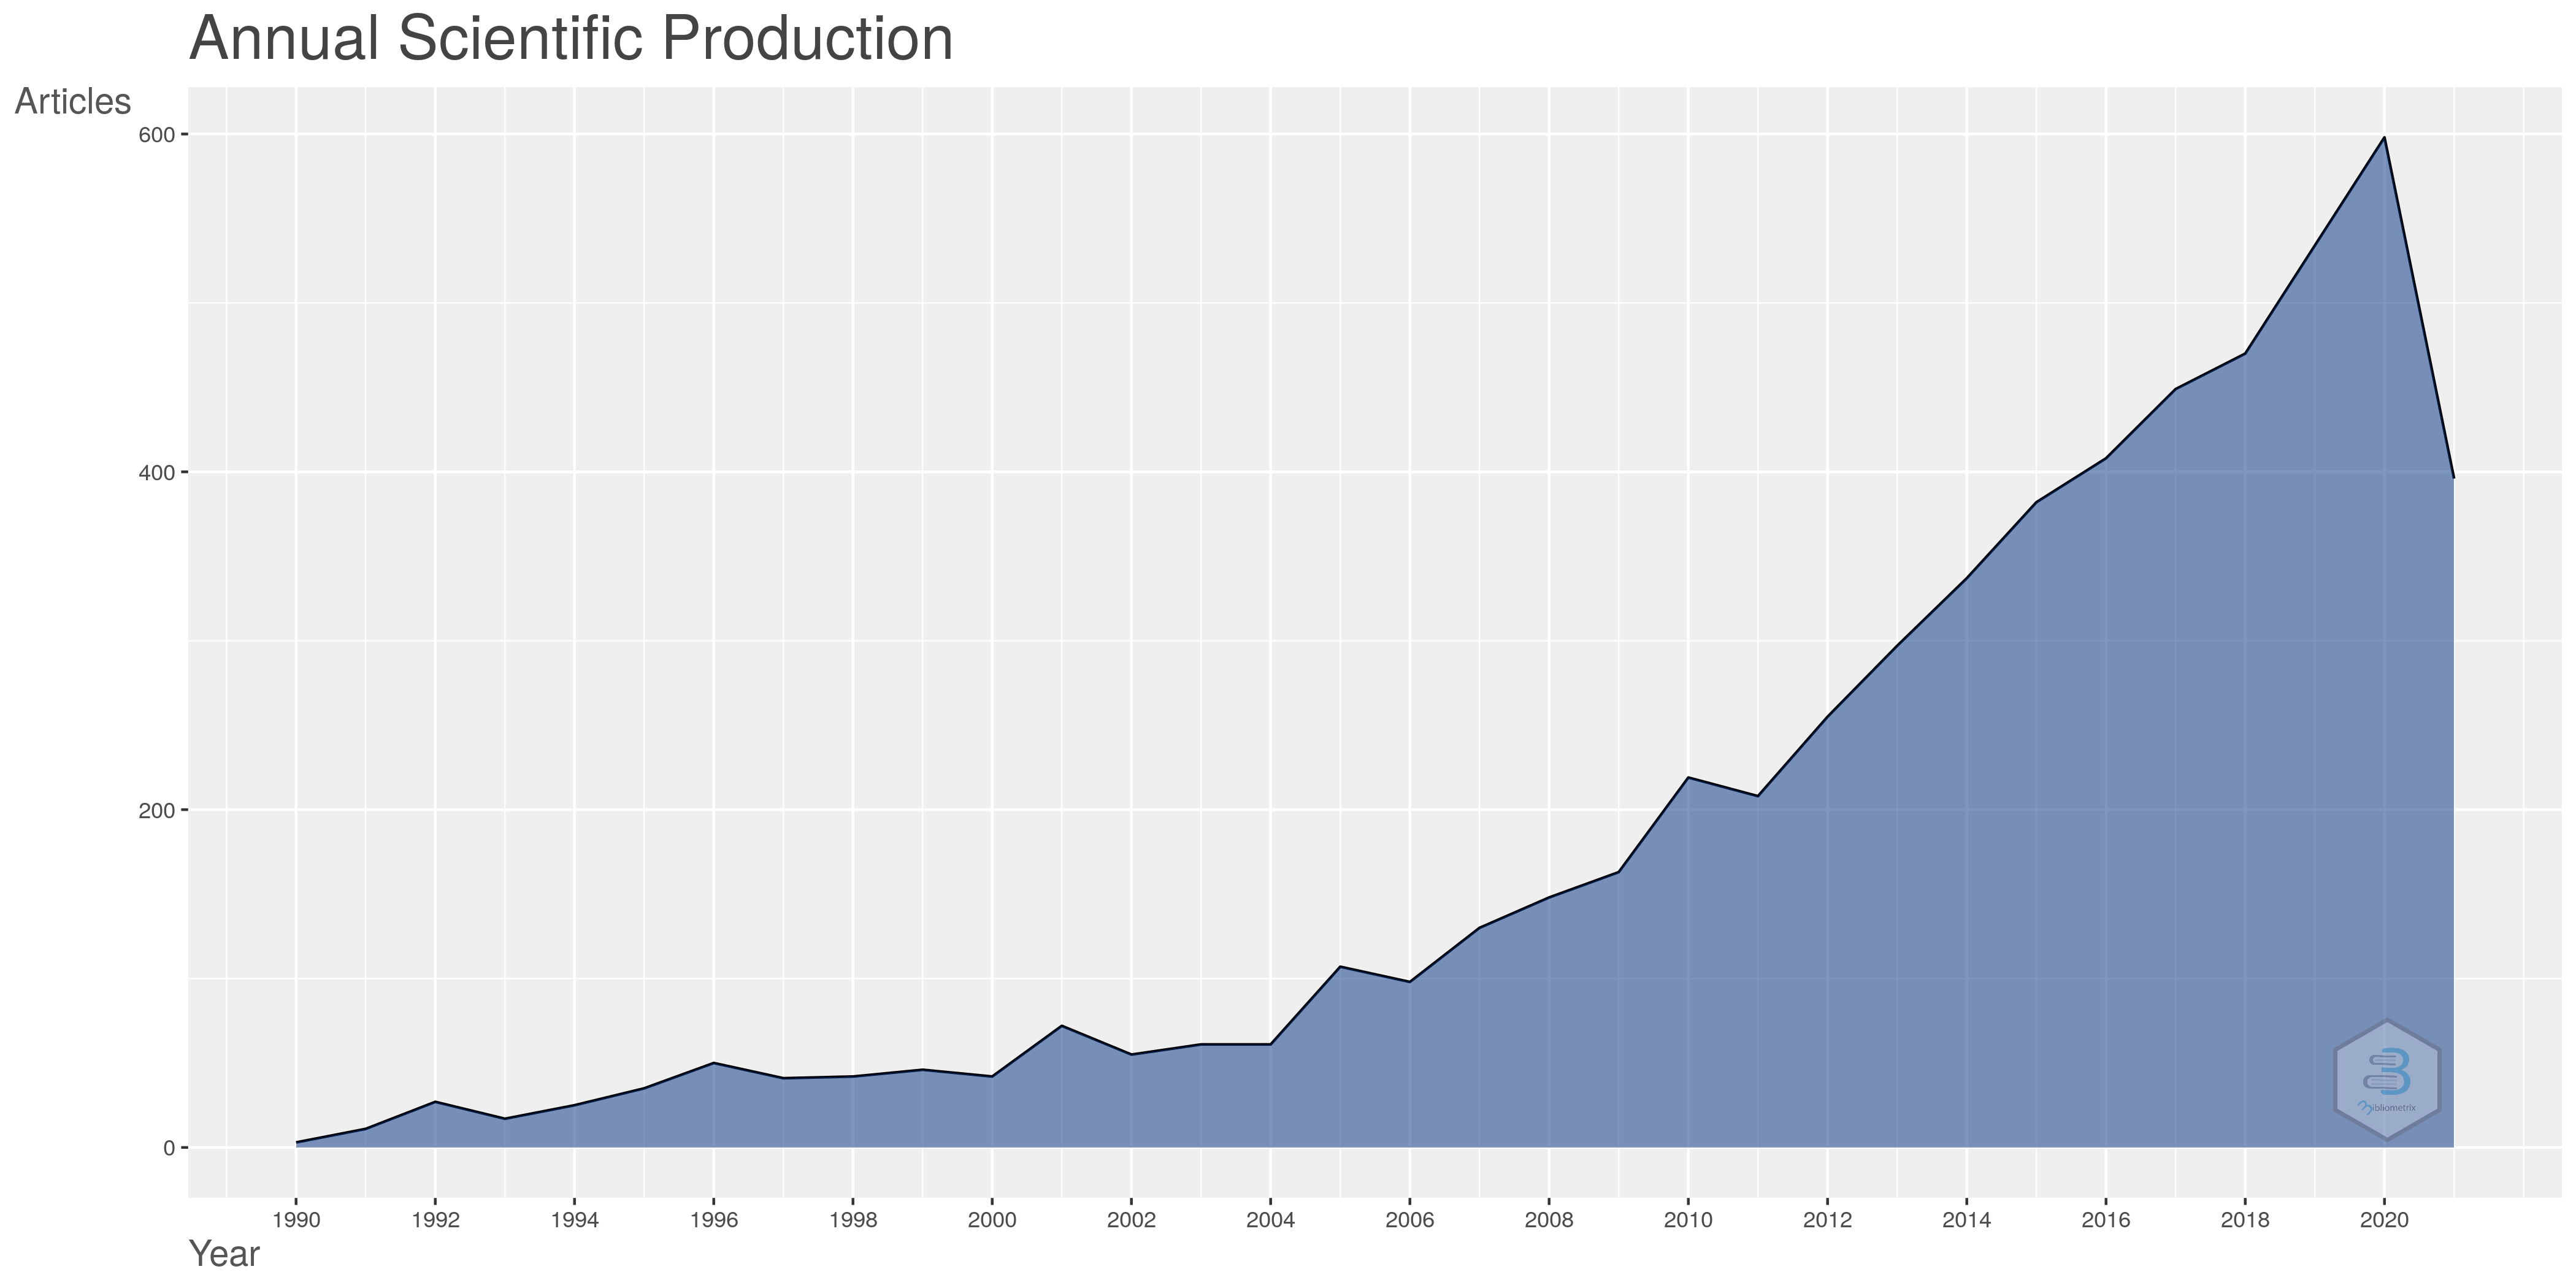
\includegraphics[width=1\textwidth]{experiments/jhcf/PesqBibliogr/SimulacaoMultiagente/WoS-20210803/classico-mais-citacoes/Dataset/AnnualScientificProduction-2021-08-05.png}
    \caption{Evolução da produção científica no \dataset\   MASSA@jhcf.}
    \label{fig:evol:anual:MASSA@jhcf}
\end{figure}

A figura \ref{fig:evol:anual:MASSA@jhcf} apresenta a evolução da produção científica mundial no tema de interesse, segundo o \dataset\   MASSA@jhcf. A curva mostra uma tendência de crescimento aproximadamente exponencial da quantidade de publicações, desde a primeira identificada em 1990.

O \textit{Annual Growth Rate} do \dataset\   é de 17,06\%, bem maior que a taxa média de crescimento da publicação científica mundial, de cerca de 3,3\% anuais, em 2016, como ilustra o estudo em \url{https://www.researchgate.net/publication/333972683_Dynamics_of_scientific_production_in_the_world_in_Europe_and_in_France_2000-2016}, página 23.

\subsection{Interpretação do Crescimento} A maior taxa de crescimento do \dataset\   MASSA@jhcf, bem como o seu grande volume, sugerem que o assunto em pauta desperta intenso interesse, inclusive de ordem econômica.

\subsection{Evolução das Citações}

\begin{figure}
    \centering
    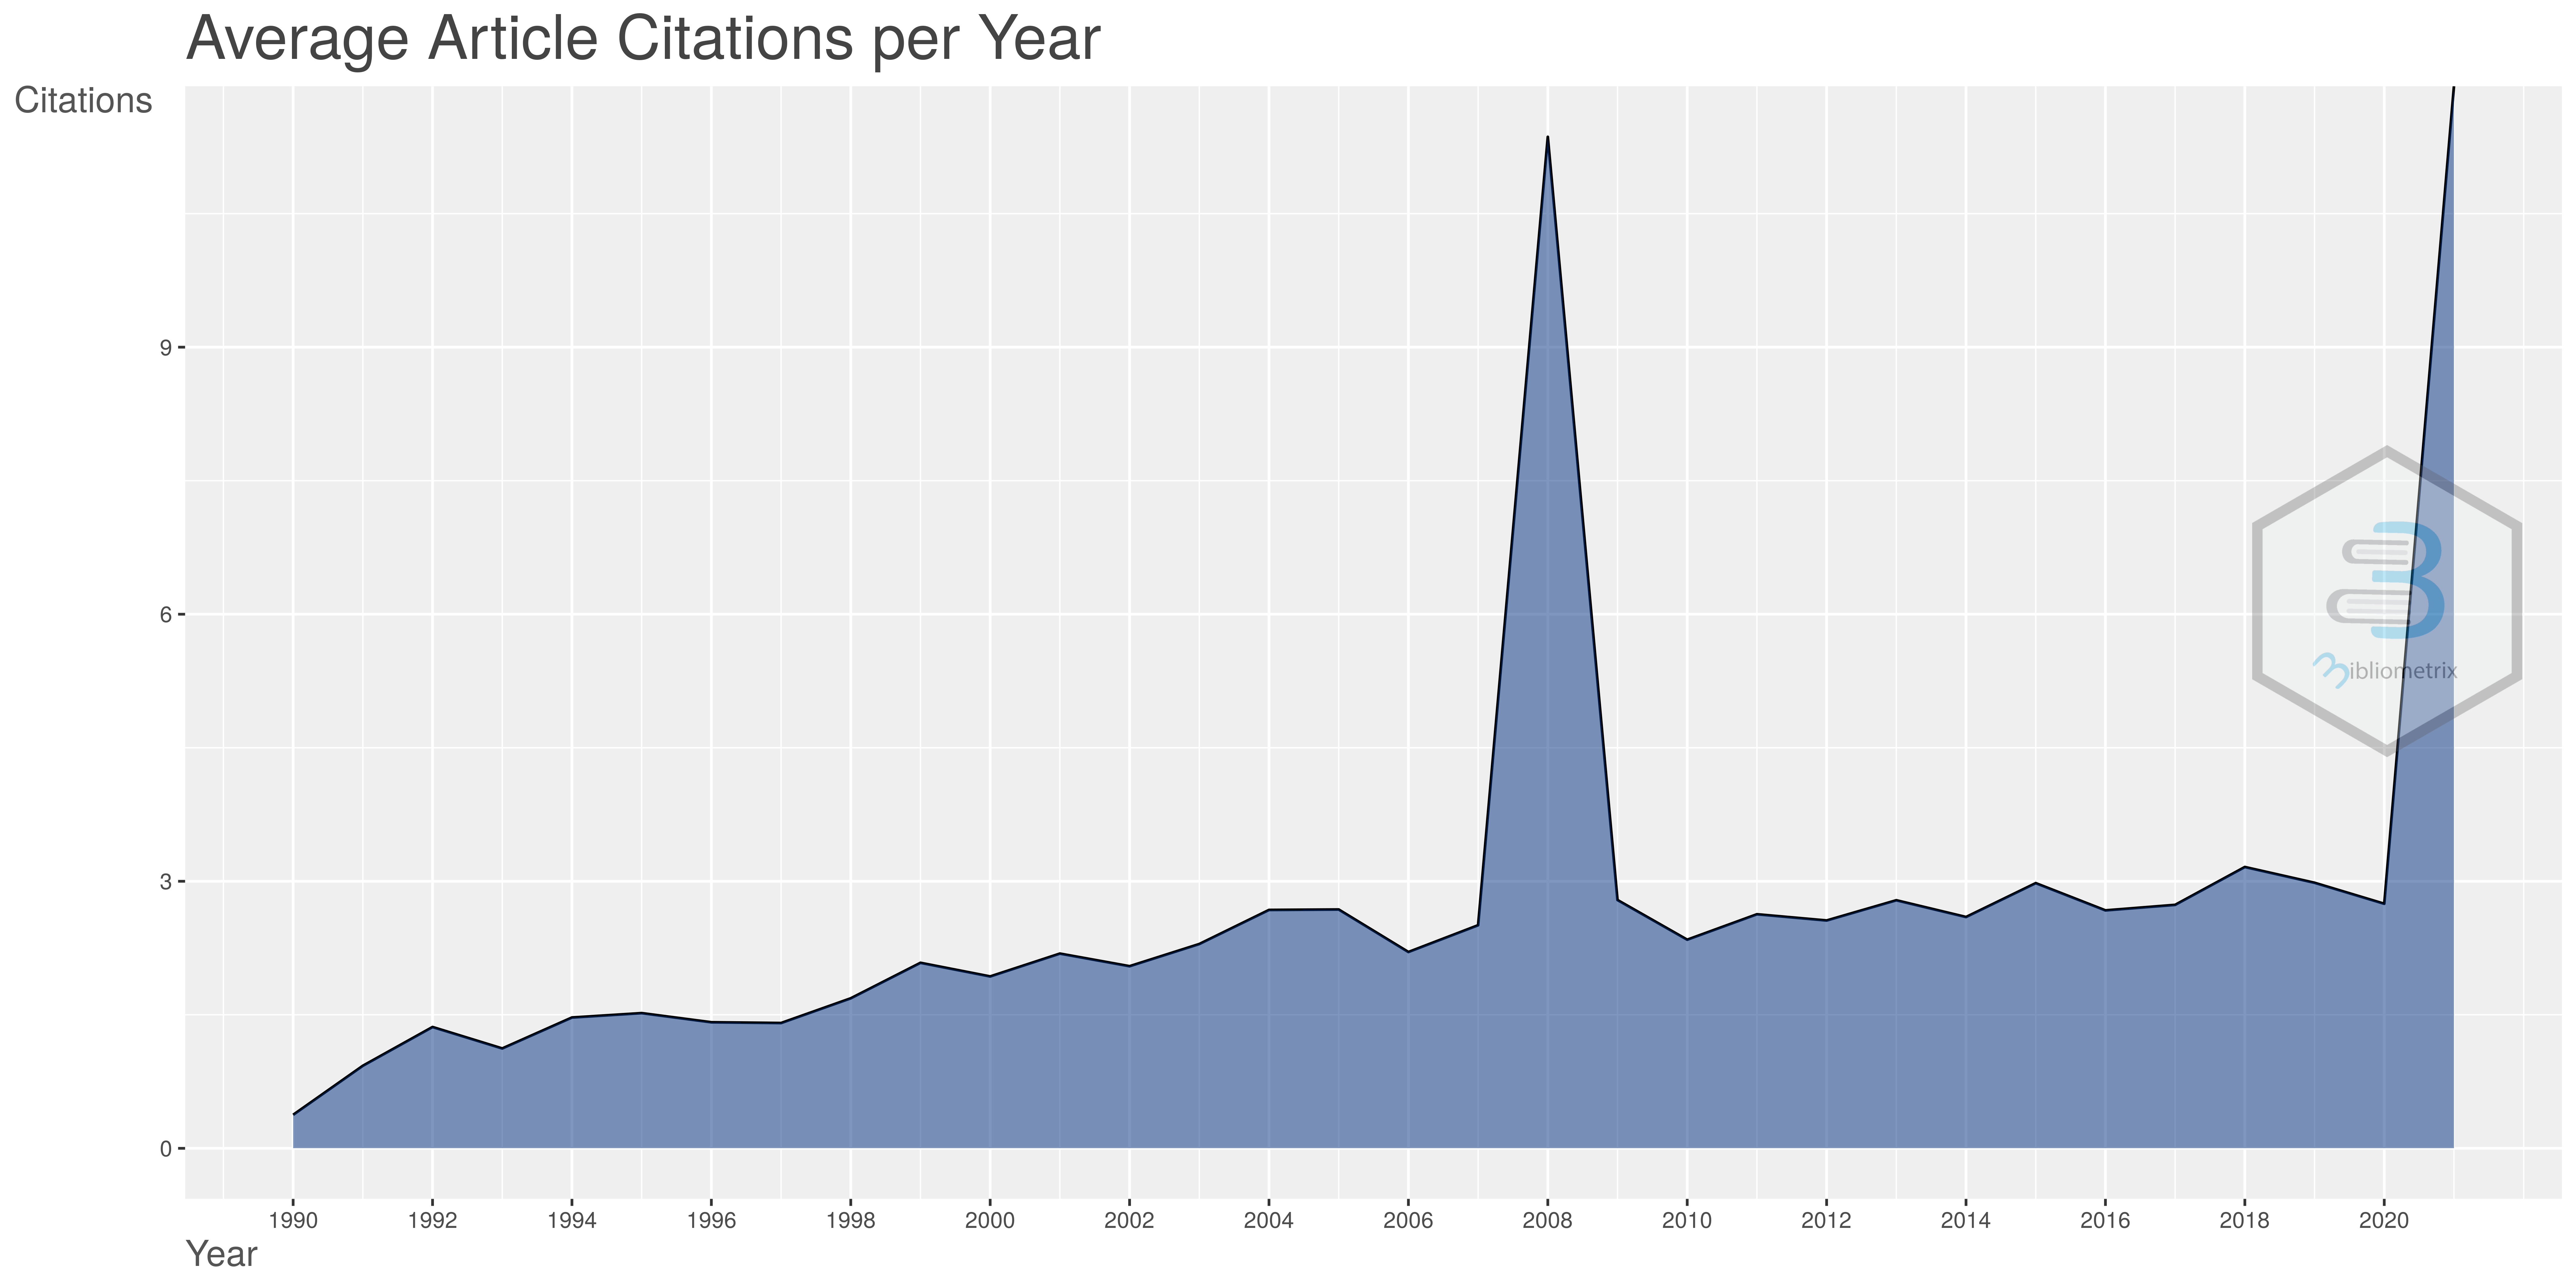
\includegraphics[width=1\textwidth]{experiments/jhcf/PesqBibliogr/SimulacaoMultiagente/WoS-20210803/classico-mais-citacoes/Dataset/AverageArticleCitationPerYear-2021-08-09.png}
    \caption{Evolução das citações ao \dataset\   MASSA@jhcf.}
    \label{fig:evol:anual:citacoes:MASSA@jhcf}
\end{figure}

A figura \ref{fig:evol:anual:citacoes:MASSA@jhcf} apresenta a evolução da média de citações aos 5.787 artigos no \dataset\   MASSA@jhcf. 
Nota-se grande estabilidade na média anual de citações, onde os artigos publicados em 1992 possuem cerca de 2 citações médias, e em 2015 (17 anos depois) o valou alterou-se apenas para três. O pico que aparece no ano de 2008 deve-se, possivelmente, à presença de um artigo do \dataset, publicado em 2008, que possui um número surpreendente grande de citações. \footnote{Note que o cálculo do número  médio de citações, nesse caso, utiliza os valores computados no tag "TC (Times Cited)", já presentes no \dataset\   obtido. Ou seja, o gráfico baseia-se no número de citações globais (externas ao \dataset\   MASSA@jhcf), e não no número de citações locais (citações a um artigo do \dataset\   feitas por alguns dos outros artigos dentro do próprio \dataset).}.

\subsection{Interpretação das Citações}
Mesmo perante um crescimento aproximadamente exponencial no volume de publicações, a ocorrência de um crescimento nas citações médias ao longo dos anos sugere que os artigos do \dataset\   possuem uma tendência de crescimento no tamanho da bibliografia citada, bem como também despertam grande interesse dos cientistas nas demais áreas do conhecimento (já que se trata de citações globais).

\subsection{\textit{Three-Field Plots (Sankey diagram)}}

As \textit{Three-Field Plots (Sankey diagram)} (plotagens do tipo ``Três Campos'') apresentam afinidades entre três conjuntos de atributos agregados que ocorrem no \dataset. Uma plotagem do tipo Sankey busca mostrar os principais fluxos entre diferentes conjuntos de itens. \footnote{Para uma introdução ver \url{https://en.wikipedia.org/wiki/Sankey_diagram}. Para obter detalhes sobre a forma de geração e utilização desse gráfico, inclusive de forma interativa, veja o vídeo em \url{https://www.youtube.com/watch?v=jBb1iha6-sg}.} 

\begin{figure}
    \centering
    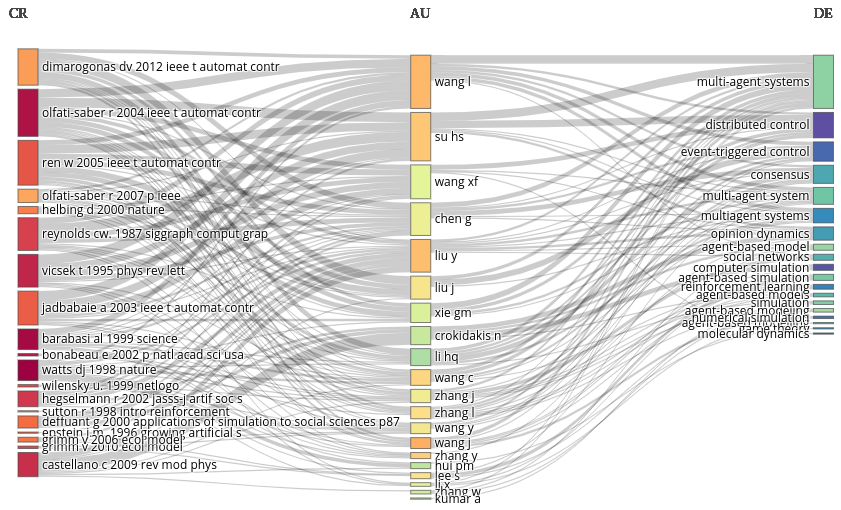
\includegraphics[angle=0,width=1\textwidth]{experiments/jhcf/PesqBibliogr/SimulacaoMultiagente/WoS-20210803/classico-mais-citacoes/Dataset/ThreeFieldPlot-AU-CR-DE-20-20-20.png}
    \caption{Plotagem ``Três Campos'' (Sankey plot) do \dataset\   MASSA@jhcf: 20 Autores, Citações e Palavras-Chave mais proeminentes.}
    \label{fig:MASSA@jhcf:ThreeFieldPlot}
\end{figure}

A figura \ref{fig:MASSA@jhcf:ThreeFieldPlot} apresenta a plotagem do tipo ``Três Campos'' do \dataset\   MASSA@jhcf, vinculando, ao centro, os 20 Autores mais proeminentes (AU), à esquerda, as 20 Citações mais frequentes (CR - Cited Records), e à direita, as 20 Palavras-Chave mais frequentes empregadas pelos autores.

\subsection{Interpretação da figura \ref{fig:MASSA@jhcf:ThreeFieldPlot}}
Os vinte autores mais relevantes, em relação aos artigos mais relevantes citados, e as palavras-chave mais relevantes são aparentemente de origem asiática, mais especificamente chinesa, com base nos sobrenomes. De outra formal, a mesma origem chinesa parece não se aplicar aos trabalhos mais citados, aparentemente europeus ou norte-americanos. Isso sugere estar ocorrendo uma migração recente da produção científica, do ocidente para o oriente. 

Adicionalmente, dentre as palavras-chave (DE) não relacionadas diretamente aos termos de busca, emergem os termos \textbf{distributed control}, \textbf{event-triggered control}, \textbf{consensus} e \textbf{opinion dynamics}. Isso sugere foco das pesquisas por autores de origem chinesa no uso de simulação multiagente voltada à compreensão dos fenômenos de controle social distribuído, formação de consenso e dinâmica da opinião (pública?).

Ainda sobre a interpretação da plotagem da figura \ref{fig:MASSA@jhcf:ThreeFieldPlot}, observa-se que os artigos mais citados encontram-se publicados pelo menos 10 anos atrás, sugerindo que não houve, nos últimos 10 anos, nenhum trabalho que tenha produzido uma mudança de paradigma no tema.
A fim de melhor evidenciar as citações mais relevantes segundo o peso dos autores e palavras-chave, o gráfico da figura \ref{fig:MASSA@jhcf:ThreeFieldPlot:10-20-20} plota apenas as 10 referências citadas, para 20 autores e palavras-chave mais proeminentes.

\begin{figure}
    \centering
    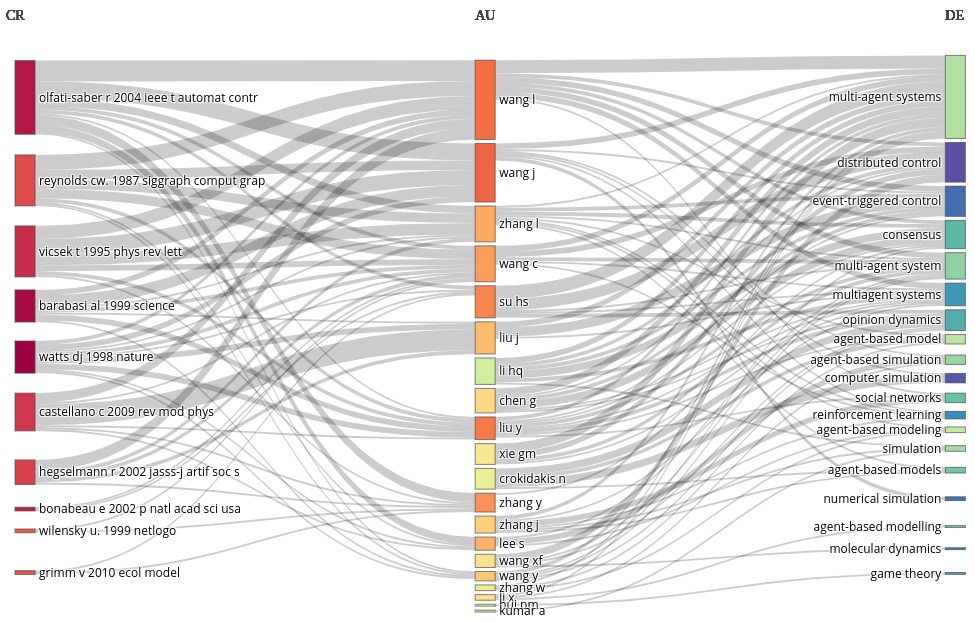
\includegraphics[angle=0,width=1\textwidth]{experiments/jhcf/PesqBibliogr/SimulacaoMultiagente/WoS-20210803/classico-mais-citacoes/Dataset/ThreeFieldPlot-AU-CR-DE-20-10-20.png}
    \caption{Plotagem ``Três Campos'' (Sankey plot) do \dataset\   MASSA@jhcf: 10 Autores, 20 Citações e Palavras-Chave mais proeminentes.}
    \label{fig:MASSA@jhcf:ThreeFieldPlot:10-20-20}
\end{figure}

Breves comentários sobre cada um desses trabalhos serão tratados em seção posterior.

\begin{itemize}
    \item  \cite{olfati-saber_consensus_2004} apresentam discussões teóricas sobre a formação de consenso em sistemas multi-agentes com topologias variáveis;
    \item  \cite{reynolds_flocks_1987} apresenta modelos multi-agentes para simulação gráfica do movimento de rebanhos ou agregados de animais.
    \item \cite{vicsek_novel_1995} analisam a emergência de fenômenos de transição de fase em simulações de de partículas com comportamento autônomo com interação biologicamente motivada.
    \item \cite{barabasi_emergence_1999} investigam a emergência da distribuição livre de escala (\textit{scale-free}\footnote{Ver introdução em \url{https://en.wikipedia.org/wiki/Scale-free_network}.}) em redes que evoluem com base em ligação preferencial.
    \item \cite{watts_collective_1998} exploram o surgimento de redes do tipo mundo pequeno (\textit{small world}\footnote{Ver introdução em \url{https://en.wikipedia.org/wiki/Small-world_network}.}) formadas a partir da reorganização aleatória de redes biológicas, genéticas e outras formas de redes auto-organizadas.
    \item \cite{castellano_statistical_2009} exploram de que forma as técnicas de análise e simulação já usadas na física-estatística podem ser usadas para explicar vários fenômenos sociais, tais como comportamento de multidões, dispersão social, comportamento de multidões etc. Eles apresentam as afinidades entre os dados gerados pelos modelos simulados e dados empíricos obtidos junto a sistemas sociais reais. 
    \item \cite{hegselmann_opinion_2002} exploram a emergência de fenômenos de consenso, polarização e fragmentação da opinião na simulação de sociedades artificiais.
    \item \cite{bonabeau_agent-based_2002} apresenta os potenciais e campos de aplicação da técnicas de simulação baseada em agentes.
    \item \cite{wilensky_netlogo_1999} apresentam a linguagem e ambiente de simulação NetLogo.
    \item \cite{grimm_standard_2006} apresenta o protocolo ODD, proposto para padronizar a descrição de modelos de simulação multiagente.
\end{itemize}

Nenhum desses 10 documentos citados está contido no \dataset\   recuperado.

%\subsection{Análises Bibliométricas: Fontes de Informação}

%\begin{figure}
%    \centering
%    \includegraphics[angle=0,width=1\textwidth]{}
%    \caption{Plotagem ``Três Campos'' (Sankey plot) do dataset MASSA@jhcf: 20 Autores, Citações e Palavras-Chave mais proeminentes.}
%    \label{fig:MASSA@jhcf:ThreeFieldPlot}
%\end{figure}

\section{Refinamento da Coleta de Dados}

No dia 03 de fevereiro de 2022, no decorrer das análises mais refinadas do \dataset\ MASSA@jhcf, identificou-se um grupo de artigos que não se encaixavam no tema de interesse, e que eram voltados para pesquisas no campo da biologia experimental e nanotecnologia. Isso sugeriu que a \query\  de busca precisaria ser reformulada, para excluir artigos que não se enquadrassem na temática desejada.
O conjunto das palavras-chave que refletia essa dissonância ficou evidente na análise da estrutura intelectual do conhecimento, do tipo \textbf{Rede de Co-ocorrências de Palavras-chave}, ilustrada no cluster em roxo, à esquerda da figura \ref{fig:MASSA@jhcf:redecoocorr-150-termos}.

\begin{figure}[htp]
    \centering
    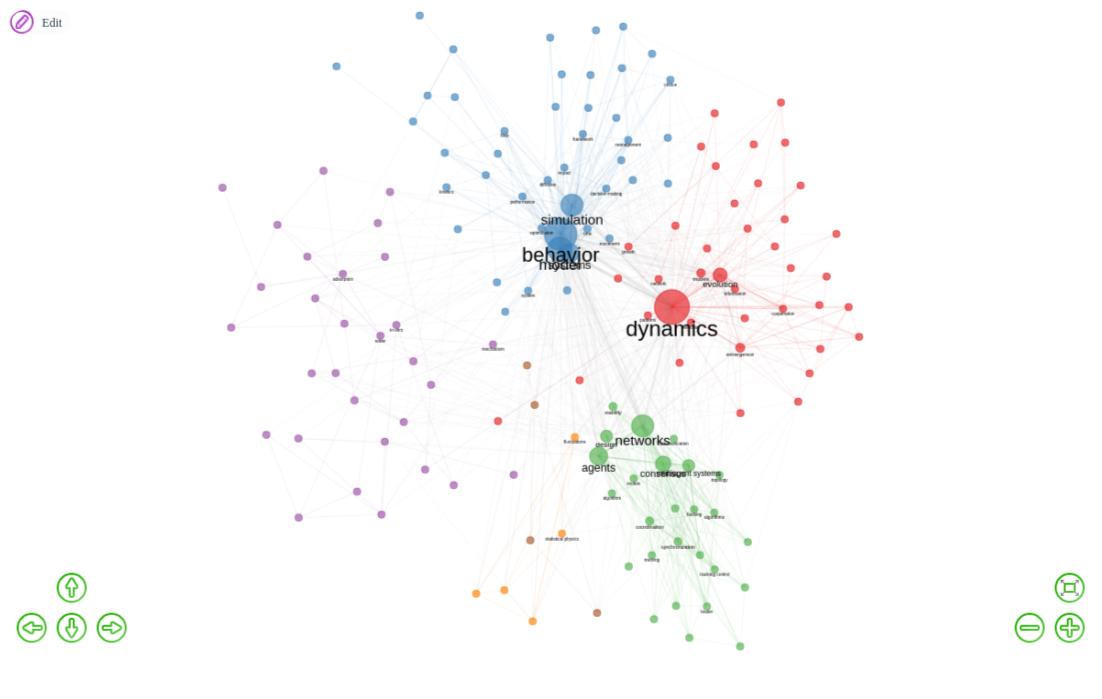
\includegraphics[clip=true,trim={9cm 0cm 7cm 0cm },width=0.6\textwidth]{experiments/jhcf/PesqBibliogr/SimulacaoMultiagente/WoS-20210803/classico-mais-citacoes/Structure-Informetric/Conceptual/Co-occurrence Network-Keywords-Plus-150-termos.png}
    \caption{Rede de co-ocorrência de palavras, com 150 termos, aplicada ao \dataset\   MASSA@jhcf.}
    \label{fig:MASSA@jhcf:redecoocorr-150-termos}
\end{figure}

As seguintes 30 palavras foram identificadas nesse \textit{cluster}:
in-vitro,
adsorption,
mechanism,
water,
force-field,
molecular-dynamics,
binding,
simulations,
nanoparticles,
bubbles,
derivatives,
temperature,
in-vivo,
mathematical-model,
oscillations,
scattering,
cancer,
contrast agents,
expression,
protein,
activation,
delivery,
surface,
removal,
acid,
agent,
reduction,
aqueous-solution,
degradation,
expectations.

Ficou evidente, pela interpretação do significado da maioria desses termos, que tais artigos não tratavam de simulação de fenômenos sociais. Isso sugere que a query está com problemas de precisão, isso é, muitos registros recuperados não atendem à necessidade de informação do pesquisador. 

Algumas dessas palavras foram então escolhidas para servir como indicativas de artigos fora do escopo, e introduzidas a partir da \query\  original, gerando uma nova \query, aprimorada e ilustrada nas linhas 1 a 13 da listagem \ref{query20220203}.

\lstinputlisting[numbers=left,basicstyle=\normalsize\ttfamily,caption={\query\  de busca sobre simulação multiagente de fenômenos socials, com ênfase em métodos experimentais, com escopo negativo de artigos que tratam de experimentos biológicos em vitro.},label=query20220203]
{experiments/jhcf/PesqBibliogr/SimulacaoMultiagente/WoS-20220203/query-Refinada.txt}

Além das justificativas para os termos usados entre as linhas 1 a 9, já descritas em \ref{MASSA:query},  justifica-se na listagem \ref{query20220203}, a inclusão da cláusula \textit{not (
 adsoption or molecular-dynamics or force-field
 or in-vitro or nanopartic* or in-vivo
 or aqueous-solution or protein or surface)}, entre as linhas 10 e 13 da \query, pois elas irão remover artigos não se enquadram no escopo da busca desejada, por usarem uma ou mais desses termos no título, resumo ou palavras-chave do artigo.
 
Usando a nova \query\ de busca, foram recuperados 6.935 documentos, que se encontram em
\url{https://github.com/jhcf/Comput-Experim-20212/experiments/jhcf/PesqBibliogr/SimulacaoMultiagente/ WoS-20220203/wos6935recs.txt}. Isso sugere que aproximadamente 1.000 registros não se enquadravam na necessidade de busca.
Uma nova análise dos dados recuperados é apresentada a seguir.

\section{Nova Análise dos Dados}

\subsection{Nova filtragem de registros}

Sobre os 6.935 documentos recuperados, foram  aplicados os seguintes filtros:
\begin{itemize}
    \item Remoção dos registros de documentos que não são artigos \textit{full paper}, isso é, artigos completos publicados em revistas;
%    \item Remoção dos registros de artigos científicos que não fazem parte do \textit{core} da bibliografa, segundo a Lei de Bradford.
\end{itemize}

Após os filtros aplicados (apenas um)  obteve-se um total de 4.647 registros, que doravante serão chamados de forma coletiva, de \dataset\   MASSA2@jhcf.

\subsection{Análise descritiva do \dataset\   MASSA2@jhcf}

\subsubsection{Dados Sumários Gerais}

\begin{table}[]
    \centering
\csvautotabular[separator=semicolon
%,filter not strcmp={\csvcolii}{}
]{experiments/jhcf/PesqBibliogr/SimulacaoMultiagente/WoS-20220203/Descritiva/MASSA2-Main-Information.csv}
    \caption{Principais dados descritivos do \dataset\   MASSA2@jhcf.}
    \label{tab:MASSA2:Main}
\end{table}

Nota-se, com os resultados da tabela \ref{tab:MASSA2:Main}, que o \dataset\   abrange um período de 32 anos de publicações (1991 a 2022), evidenciando  a publicação dos 4.647 artigos em 1.910 revistas distintas. Esses artigos tem idade média de publicação de 7.8.

Adicionalmente, o \dataset\ apresenta 157.507 referências citadas, com uma média de (157.507/4.647 = ?) 33,89 referências citadas por artigo.

14.229 autores distintos produziram os artigos, com uma média de 3,73 autores por documento.

\subsubsection{Evolução anual da produção científica}

No tema de simulação multiagente de fenômenos sociais, a evolução anual da produção científica mundial é sumarizada no gráfico da figura \ref{fig:MASSA2:Evolucao}.

\begin{figure}
    \centering
    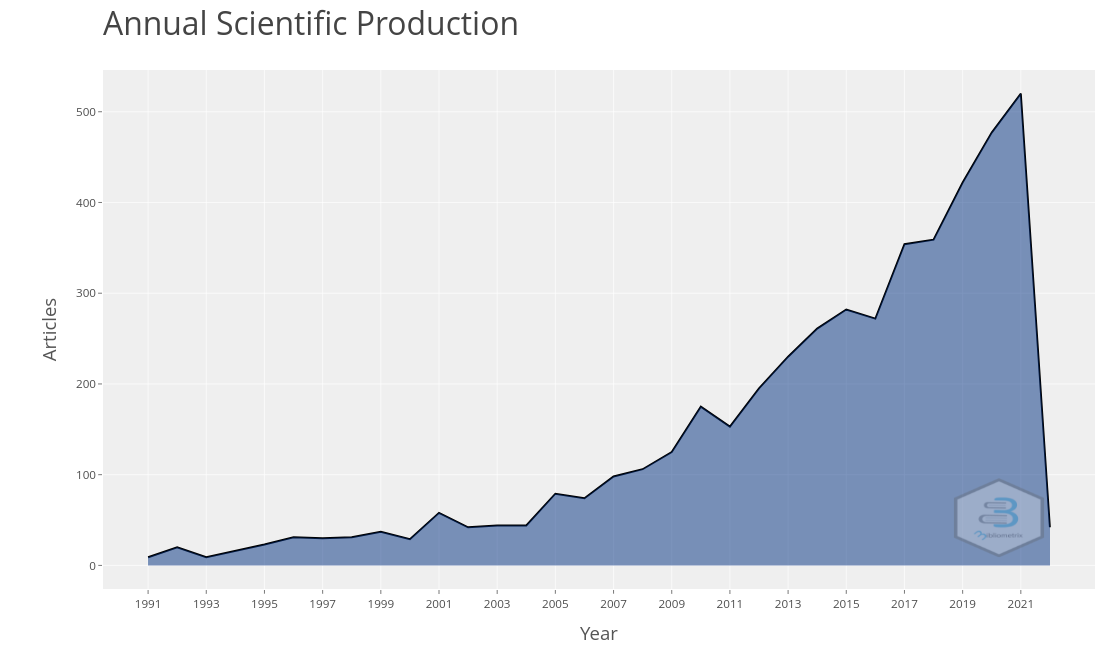
\includegraphics[width=1\textwidth]{experiments/jhcf/PesqBibliogr/SimulacaoMultiagente/WoS-20220203/Descritiva/MASSA2-Annual-Scientific-Production.png}
    \caption{Evolução da Produção Científica Anual, segundo o \dataset\ MASSA2@jhcf.}
    \label{fig:MASSA2:Annual-Scientific-Production}
\end{figure}

Entre 1991 e 2005 o crescimento de publicações era quase linear. As publicações mostram-se em ascendência forte a partir dos últimos seis anos (2015). Esse crescimento tem sido visto em várias outras áreas de conhecimento.

\subsubsection{Média de citações anuais por artigo}

O gráfico da figura \ref{fig:MASSA2:Media:Citacoes} apresenta a evolução das citações anuais médias, para os artigos do \dataset\ MASSA2@jhcf. Observa-se que há um crescimento discreto da média, onde os artigos mais recentes tendem a ser mais citados, como esperado. A redução da média no ano de 2021 deve-se, provavelmente, à insuficiência de indexação e de citação para os artigos mais recentes, tendo em vista que p ano de 2021 foi encerrado há menos de dois meses. 

\begin{figure}
    \centering
    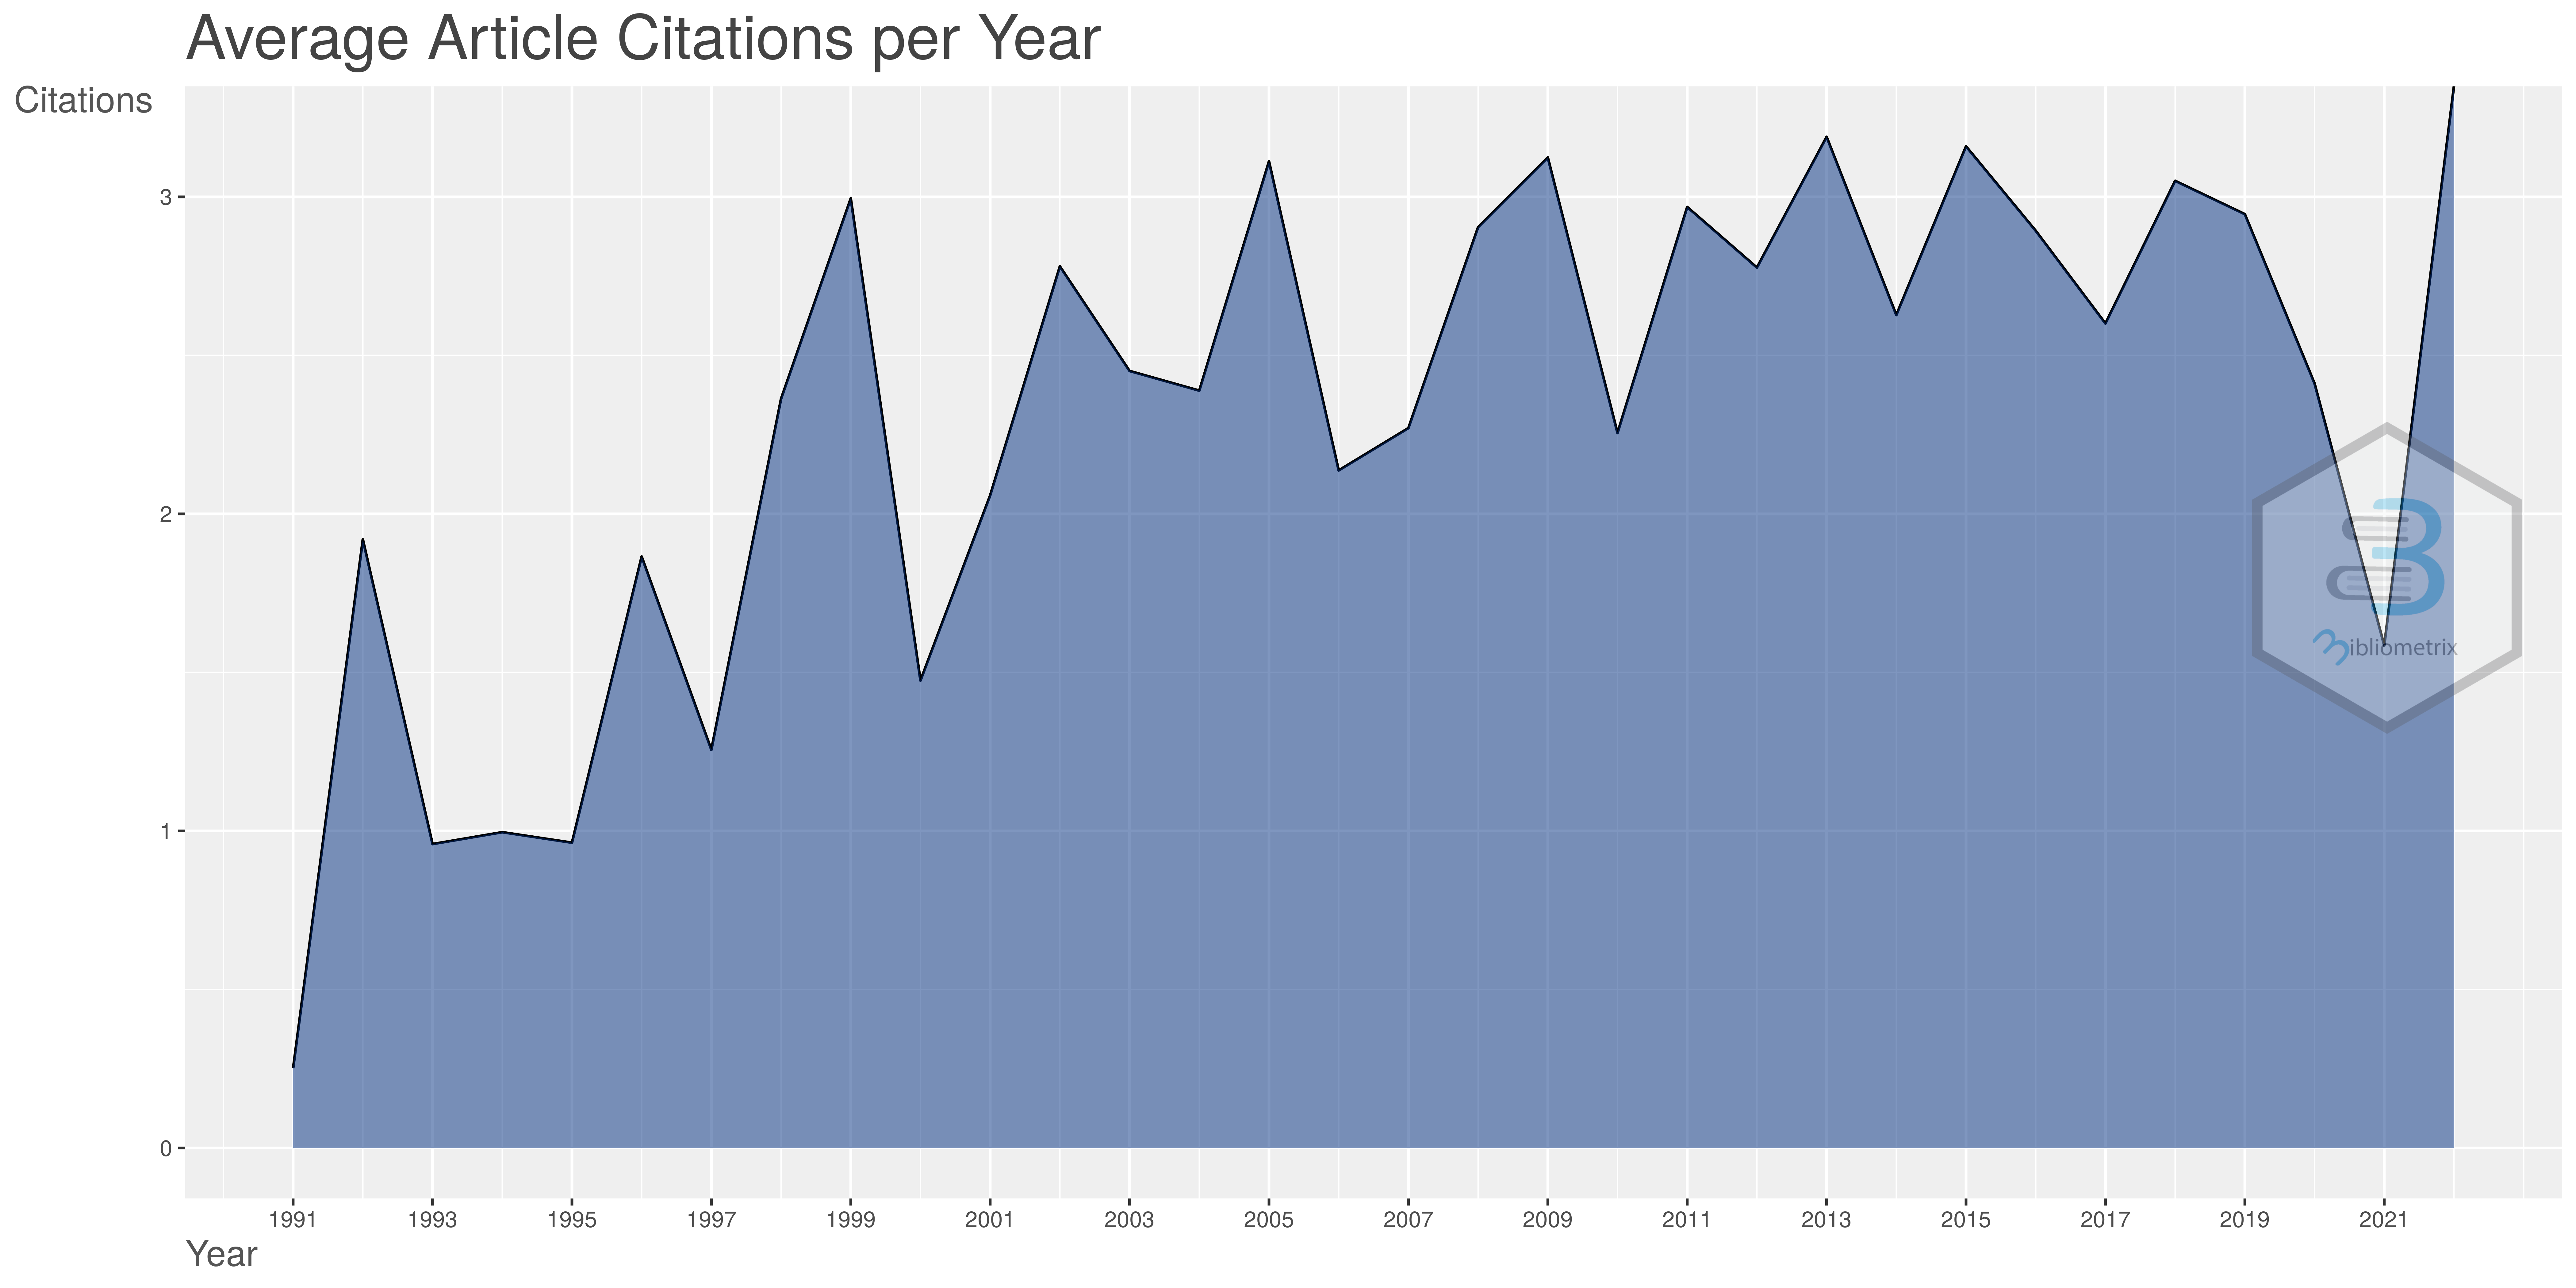
\includegraphics[width=1\textwidth]{experiments/jhcf/PesqBibliogr/SimulacaoMultiagente/WoS-20220203/Descritiva/MASSA2-Average-Citations-per-Year.png}
    \caption{Média de citações para cada artigo do \dataset\ MASSA2@jhcf, conforme o ano de publicação}
    \label{fig:MASSA2:Media:Citacoes}
\end{figure}

Para que melhor se compreenda como foi produzido o gráfico, a tabela \ref{tab:MASSA2:Media:Citacoes} apresenta parcialmente os dados de citação anual para os artigos do \dataset\ MASSA2@jhcf. A título de exemplo, nota-se que no \dataset\ foram encontrados 9 artigos publicados no ano de 1991, tendo sido cada artigo citado, em média, aproximadamente 31,4 vezes. Dado que esses artigos já tem 31 anos citáveis, obtém-se uma média de 1,01 citações anuais, aproximadamente.

\begin{table}[]
    \centering
\csvautotabular[separator=semicolon
%,filter not strcmp={\csvcolii}{}
]{experiments/jhcf/PesqBibliogr/SimulacaoMultiagente/WoS-20220203/Descritiva/MASSA2-Average-Citations-per-Year.csv}
    \caption{Dados parciais de citação anual para os artigos do \dataset\   MASSA2@jhcf.}
    \label{tab:MASSA2:Media:Citacoes}
\end{table}

\subsubsection{Diagramas de Sankey (\textit{three fields plots})} 

A fim de apresentar mais alguns dados sumários gerais sobre  o \dataset, as figuras \ref{fig:MASSA2:Sankey:CR-AU-DE} e \ref{fig:MASSA2:Sankey:SO:DE:AU_UN} apresentam plotagens do tipo 
\textit{three fields plots}, também conhecidas pelo nome de Diagramas de Sankey \citep{riehmann_interactive_2005}, que possibilitam várias combinações de afinidades mais evidentes entre as diversas colunas dos registros do \dataset.

A primeira plotagem, figura \ref{fig:MASSA2:Sankey:CR-AU-DE}, apresenta as afinidades mais evidentes entre 15 Autores (centro), 15 Palavras-chave (direita) e 15 Referências citadas (esquerda). Ao centro, observa-se que os autores mais evidentes, segundo a técnica apresentada, tem origem asiática, a julgar pelos nomes. 

As 15 palavras-chave mais evidentes sugerem que o \dataset\ possui artigos que refletem a busca sobre o tema desejado, mas que há muitas palavras distintas que representam o mesmo conceito, como as a seguir listadas:
\begin{enumerate}
    \item multi-agent systems;
    \item multiagent system;
    \item multiagent system; 
    \item agent-based model;  
    \item agent-based models;
    \item agent-based modeling;
    \item agent-based simulation;
\end{enumerate}

As cinco palavras a seguir sugerem, o que pode ser comprovado com o aprofundamento desse estudo bibliográfico, que o estado da arte no tema busca atualmente respostas, ou possui fundamentos nas seguintes questões:
\begin{description}
    \item [event-triggered control] Como eventos disparadores exercem  controle sobre o comportamento (coletivo) de grupos sociais?
    \item [consensus] Como usar simulação multi-agente para entender o surgimento de consenso em grupos sociais?
    \item [opinion dynamics] Como usar simulação multi-agente para entender a dinâmica de opiniões que se formam em grupos sociais?
    \item [social networks] Como os métodos da análise de redes sociais podem ser usados no tema da simulação multiagente?
    \item [reinforcement learning] Como usar os métodos e técnicas de aprendizagem por reforço em simulação multiagente?
    \item [game theory] Como usar os métodos e técnicas da teoria dos jogos em simulação multiagente?
\end{description}

Algumas das referências citadas, apresentadas à esquerda do gráfico, devem evidenciar a pertinência das questões acima sugeridas, a ser comprovado até o final do estudo. 

\begin{figure}
    \centering
    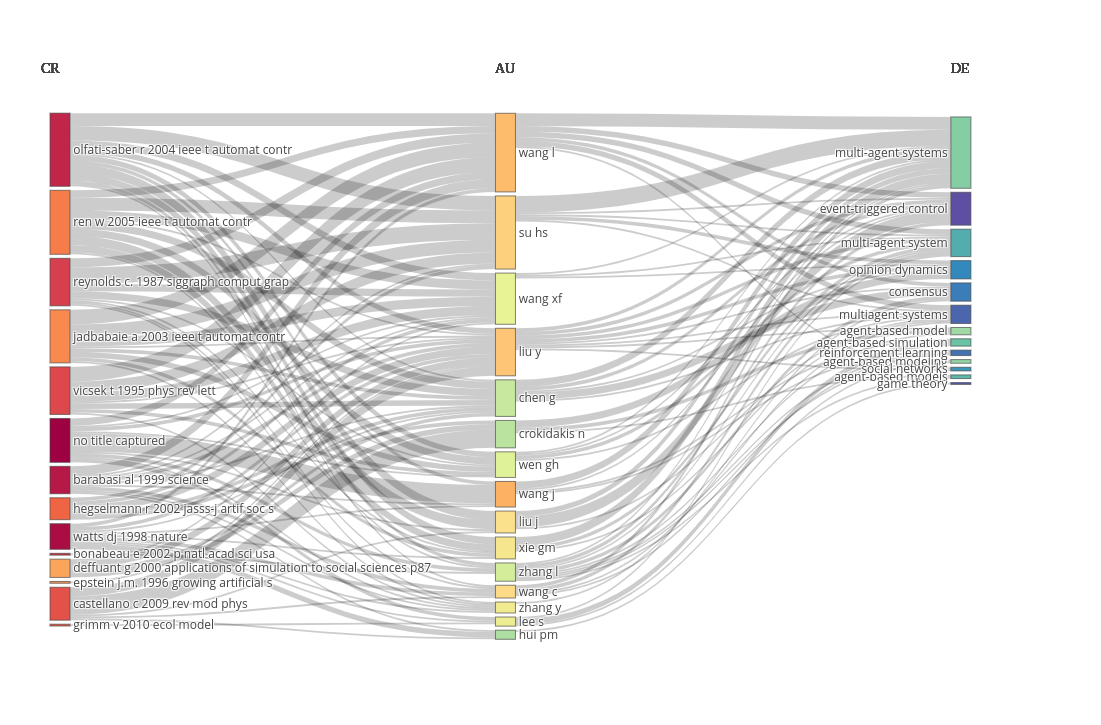
\includegraphics[angle=90,width=1\textwidth,height=0.9\textheight]{experiments/jhcf/PesqBibliogr/SimulacaoMultiagente/WoS-20220203/Descritiva/MASSA2-Three-Fields-Plot-CR-AU-DE.png}
    \caption{Diagrama Sankey, relacionando as afinidades mais evidentes entre Autores (centro), Palavras-chave (direita) e Referências citadas (esquerda).}
    \label{fig:MASSA2:Sankey:CR-AU-DE}
\end{figure}

A segunda plotagem, figura \ref{fig:MASSA2:Sankey:SO:DE:AU_UN}, apresenta as afinidades mais evidentes entre 15 revistas (esquerda), 15 palavras-chave (centro) e 15 instituições de filiação dos autores (direita). Com base na técnica usada, fica evidente a proeminência dos seguintes \textit{journals} sobre os demais, sendo apresentado um breve trecho do foco de cada revista, extraído da página online da revista:
\begin{itemize}
    \item JASSS: The Journal of Artificial Societies and Social Simulation. \textit{\small  is an interdisciplinary journal for the exploration and understanding of social processes by means of computer simulation. Since its first issue in 1998, it has been a world-wide leading reference for readers interested in social simulation and the application of computer simulation in the social sciences.}. Fonte \url{https://www.jasss.org/admin/about.html};
    \item PHYSICA A-STATISTICAL MECHANICS AND ITS APPLICATIONS. \textit{\small ... publishes research in the field of statistical mechanics and its applications. Statistical mechanics sets out to explain the behaviour of macroscopic systems, or the large scale, by studying the statistical properties of the microscopic or nanoscopic constituents. Applications of the concepts and techniques of statistical mechanics include: applications to physical and physiochemical systems such as solids, liquids and gases, interfaces, glasses, colloids, complex fluids, polymers, complex networks, applications to economic and social systems (e.g. socio-economic networks, financial time series, agent based models, systemic risk, market dynamics, computational social science, science of science, evolutionary game theory, cultural and political complexity), and traffic and transportation (e.g. vehicular traffic, pedestrian and evacuation dynamics, network traffic, swarms and other forms of collective transport in biology, models of intracellular transport, self-driven particles), as well as biological systems (biological signalling and noise, biological fluctuations, cellular systems and biophysics); and other interdisciplinary applications such as artificial intelligence (e.g. deep learning, genetic algorithms or links between theory of information and thermodynamics/statistical physics.).}. Fonte: \url{https://www.journals.elsevier.com/physica-a-statistical-mechanics-and-its-applications};
    \item IEEE ACCESS. \textit{\small ... is a multidisciplinary, all-electronic archival journal, continuously presenting the results of original research or development across all IEEE’s fields of interest. Supported by article processing charges (APC), its hallmarks are a rapid peer review and publication process of 4 to 6 weeks, with open access to all readers.}. Fonte: \url{https://ieeeaccess.ieee.org/about-ieee-access/learn-more-about-ieee-access/}
\end{itemize} 

\begin{figure}
    \centering
    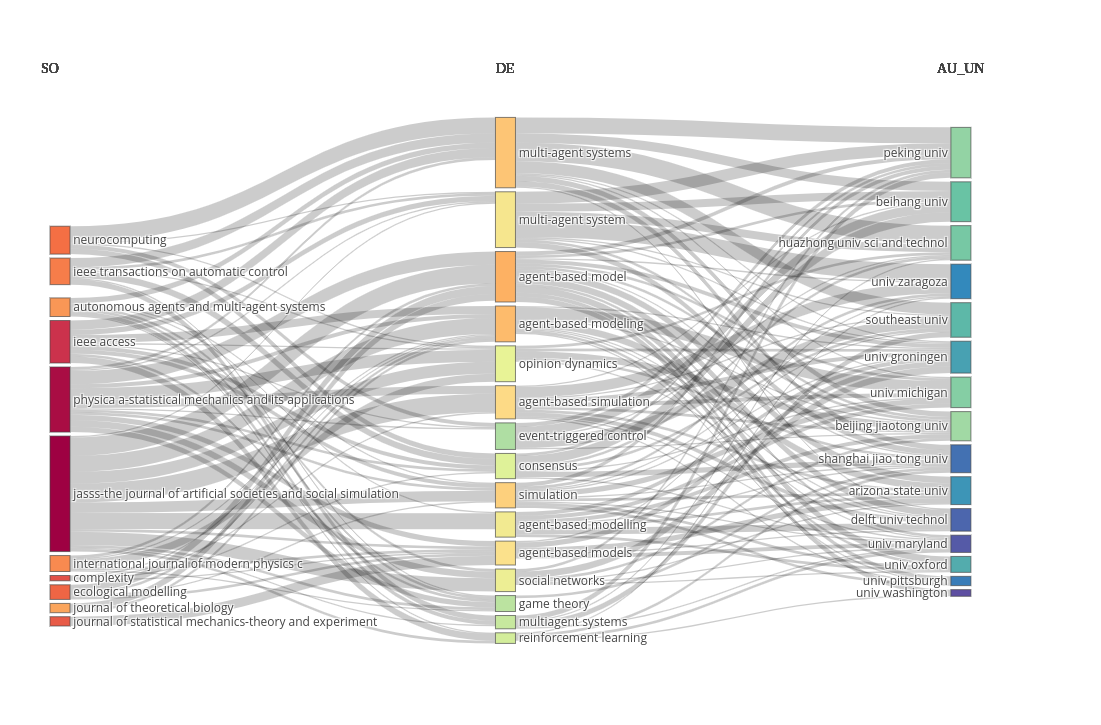
\includegraphics[angle=90,width=1\textwidth,height=0.9\textheight]{experiments/jhcf/PesqBibliogr/SimulacaoMultiagente/WoS-20220203/Descritiva/MASSA2-Three-Fields-Plot-SO:DE:AU_UN.png}
    \caption{Diagrama Sankey, relacionando as afinidades mais evidentes entre revistas (esquerda), palavras-chave (centro) e instituição de filiação dos autores (direita).}
    \label{fig:MASSA2:Sankey:SO:DE:AU_UN}
\end{figure}

Observa-se, com base no escopo declarado de cada uma das revistas, que a revista JASSS é bem enquadrada no escopo da busca, enquanto que a revista IEEE Access não tem relação direta com o tema. Já a revista Physica A aborda o tema de forma mais ampla do que o buscado, com ênfase em métodos da mecânica estatística, que não são os únicos possíveis de serem empregados.
Os nomes das demais 8 revistas, apresentadas no diagrama, são os seguintes:
\begin{enumerate}
    \item NEUROCOMPUTING \textit{\small  ... welcomes theoretical contributions aimed at winning further understanding of neural networks and learning systems, including, but not restricted to, architectures, learning methods, analysis of network dynamics, theories of learning, self-organization, biological neural network modelling, sensorimotor transformations and interdisciplinary topics with artificial intelligence, artificial life, cognitive science, computational learning theory, fuzzy logic, genetic algorithms, information theory, machine learning, neurobiology and pattern recognition.}. Fonte: \url{https://www.journals.elsevier.com/neurocomputing};
    \item IEEE TRANSACTIONS ON AUTOMATIC CONTROL \textit{\small publishes high-quality papers on the theory, design, and applications of control engineering.  Two types of contributions are regularly considered: 
1) Papers:  Presentation of significant research, development, or application of control concepts. 
2) Technical Notes and Correspondence:  Brief technical notes, comments on published areas or established control topics, corrections to papers and notes published in the Transactions.
In addition, special papers (tutorials, surveys, and perspectives on the theory and applications of control systems topics) are solicited. }. Fonte: \url{https://ieeexplore.ieee.org/xpl/aboutJournal.jsp?punumber=9};
    \item AUTONOMOUS AGENTS AND MULTI-AGENT SYSTEMS \textit{\small is the official journal of the International Foundation for Autonomous Agents and Multi-Agent Systems. It provides a leading forum for disseminating significant original research results in the foundations, theory, development, analysis, and applications of autonomous agents and multi-agent systems. Coverage in Autonomous Agents and Multi-Agent Systems includes, but is not limited to:
Agent decision-making architectures and their evaluation, including: cognitive models; knowledge representation; logics for agency; ontological reasoning; planning (single and multi-agent); reasoning (single and multi-agent)
Cooperation and teamwork, including: distributed problem solving; human-robot/agent interaction; multi-user/multi-virtual-agent interaction; coalition formation; coordination
Agent communication languages, including: their semantics, pragmatics, and implementation; agent communication protocols and conversations; agent commitments; speech act theory
Ontologies for agent systems, agents and the semantic web, agents and semantic web services, Grid-based systems, and service-oriented computing
Agent societies and societal issues, including: artificial social systems; environments, organizations and institutions; ethical and legal issues; privacy, safety and security; trust, reliability and reputation
Agent-based system development, including: agent development techniques, tools and environments; agent programming languages; agent specification or validation languages
Agent-based simulation, including: emergent behavior; participatory simulation; simulation techniques, tools and environments; social simulation
Agreement technologies, including: argumentation; collective decision making; judgment aggregation and belief merging; negotiation; norms
Economi c paradigms, including: auction and mechanism design; bargaining and negotiation; economically-motivated agents; game theory (cooperative and non-cooperative); social choice and voting
Learning agents, including: computational architectures for learning agents; evolution, adaptation; multi-agent learning.
Robotic agents, including: integrated perception, cognition, and action; cognitive robotics; robot planning (including action and motion planning); multi-robot systems.
Virtual agents, including: agents in games and virtual environments; companion and coaching agents; modeling personality, emotions; multimodal interaction; verbal and non-verbal expressiveness
Significant, novel applications of agent technology
Comprehensive reviews and authoritative tutorials of research and practice in agent systems
Comprehensive and authoritative reviews of books dealing with agents and multi-agent systems.
Official journal of the International Foundation for Autonomous Agents and Multi-Agent Systems.
Covers the foundations, theory, development, analysis, and applications of autonomous agents and multi-agent systems.
Presents comprehensive reviews and authoritative tutorials of research and practice in agent systems.}. Fonte: \url{https://www.springer.com/journal/10458};
    \item INTERNATIONAL JOURNAL OF MODERN PHYSICS C \textit{\small is a journal dedicated to Computational Physics and aims at publishing both review and research articles on the use of computers to advance knowledge in physical sciences and the use of physical analogies in computation. Topics covered include: algorithms; computational biophysics; computational fluid dynamics; statistical physics; complex systems; computer and information science; condensed matter physics, materials science; socio- and econophysics; data analysis and computation in experimental physics; environmental physics; traffic modelling; physical computation including neural nets, cellular automata and genetic algorithms.}. Fonte: \url{https://www.worldscientific.com/page/ijmpc/aims-scope};
    \item COMPLEXITY \textit{\small The purpose of Complexity is to report important advances in the scientific study of complex systems. Complex systems are characterized by interactions between their components that produce new information — present in neither the initial nor boundary conditions — which limit their predictability. Given the amount of information processing required to study complexity, the use of computers has been central to complex systems research. Concepts relevant to Complexity include:
    Adaptability, robustness, and resilience;
    Complex networks;
    Criticality;
    Evolution and emergent behaviour;
    Nonlinear dynamics;
    Pattern formation;
    Self-organization.
Methods used within the scientific study of complex systems frequently include:
    Agent-based modelling;
    Analytical methods;
    Cellular automata;
    Computational methods;
    Data science;
    Game theory;
    Machine learning;
    Statistical mechanics.
Applications of complex systems may be related to the following disciplines, among others:
Computational social science;    Digital epidemiology;
    Ecology;
    Economics;
    Engineering;
    Socio-technical systems;
    Statistical linguistics;
    Systems biology;
    Urban systems.}. Fonte: \url{https://www.hindawi.com/journals/complexity/about/};
    \item ECOLOGICAL MODELLING \textit{\small publishes new mathematical models and systems analysis for describing ecological processes, and novel applications of models for environmental management.
We welcome research on process-based models embedded in theory with explicit causative agents and innovative applications of existing models. And because applications can help refine models and propose new directions for research, the journal publishes both to help foster reproducibility and utility.Human activity and well-being are dependent on and integrated with the functioning of ecosystems and the services they provide. We aim to understand these basic ecosystem functions using mathematical and conceptual modelling, systems analysis, thermodynamics, computer simulations, and ecological theory, and look to a wide spectrum of applications ranging from basic ecology to human ecology to socio-ecological systems. The journal welcomes original research articles, review articles, viewpoint articles and short communications.}. Fonte: \url{https://www.journals.elsevier.com/ecological-modelling};
    \item JOURNAL OF THEORETICAL BIOLOGY \textit{\small is the leading forum for theoretical perspectives that give insight into biological processes. It covers a very wide range of topics and is of interest to biologists in many areas of research, including:
Brain and Neuroscience;
Cancer Growth and Treatment;
Cell Biology;
Developmental Biology;
Ecology;
Evolution;
Immunology;
Infectious and non-infectious Diseases;
Mathematical, Computational, Biophysical and Statistical Modeling;
Microbiology, Molecular Biology, and Biochemistry;
Networks and Complex Systems;
Physiology;
Pharmacodynamics;
Animal Behavior and Game Theory}. Fonte: \url{https://www.journals.elsevier.com/journal-of-theoretical-biology};
    \item JOURNAL OF STATISTICAL MECHANICS-THEORY AND EXPERIMENT \textit{\small is targeted to a broad community interested in different aspects of statistical physics, which are roughly defined by the fields represented in the conferences called 'Statistical Physics'. Submissions from experimentalists working on all the topics which have some 'connection to statistical physics are also strongly encouraged.
The journal covers different topics which correspond to the following keyword sections:
Quantum statistical physics, condensed matter, integrable systems;
Classical statistical mechanics, equilibrium and non-equilibrium;
Disordered systems, classical and quantum;
Interdisciplinary statistical mechanics;
Biological modelling and information}. Fonte: \url{https://iopscience.iop.org/journal/1742-5468/page/about_the_journal}.
\end{enumerate}
Considerando a possibilidade de pertinência da questão ecológica ao tema dos sistemas multi-agentes, todos os \textit{journals} identificados apresentam pertinência às perguntas de pesquisa formuladas. 

Acerca das instituições de filiação dos autores, nota-se que 1/3 delas é localizada na china, 1/3 nos EUA, e o restante na Europa e Austrália. É provável que muitos pesquisadores de origem chinesa trabalhem em universidades fora da china, no tema do \dataset.


\subsection{Medidas bibliométricas}

As medidas bibliométricas propriamente ditas, relativas ao \dataset\ MASSA2@jhcf, serão exploradas nesta subseção, e são organizadas em três conjuntos:
\begin{description}
    \item [Relativas às Fontes de Informação] Uma vez que foram consideradas apenas as publicações em revistas, todas as fontes de informação mensuradas serão revistas científicas, ou \textit{journals}. As principais medidas são de impacto das fontes, mensuradas com base no número de citações que os artigos publicados nas revistas obtiveram de outras publicações, possivelmente feitas em outras fontes de informação, como outras revistas, seções de livros, artigos de conferência etc. As citações são registradas pelas organizações que fazem indexação de artigos, como a Web of Science e SCOPUS;
    \item [Relativas aos Autores] Sempre que um artigo publicado por um ou mais autores e também indexado por uma organização (Web of Science,  SCOPUS etc), é citado em um outro artigo também indexado por essa mesma organização, então é feita a anotação de uma citação ao mesmo, e o impacto potencial desse autor sobre a ciência é atestado pelo valor mais alto da citação do conjunto de seus artigos indexados. Várias métricas (índice H, G, M etc) podem ser derivadas dessa medida (quantidade de citações), e são exploradas tanto em relação aos autores como em relação às revistas onde esses artigos foram publicados;
    \item [Relativas aos Documentos] Cada citação adicional a  um documento (artigo de revista, de conferência, livro, ou  capítulo de livro) é um indicador do impacto do documento em si, que evidencia a sua importância. Além das citações, a ocorrência de palavras dentro dos documentos, inclusive ordenada pelo tempo, também produz indicadores numéricos (métricas) relevantes para analisar a importância do documento em relação a outros. 
\end{description}

Essas medidas serão apresentadas a seguir.

\subsubsection{Bibliometrias aplicadas aos documentos (Artigos científicos) no \dataset}

\paragraph{Citações globais aos artigos no \dataset}

Cada registro recuperado no \dataset\ apresenta um conjunto de informações, dentre as quais pode constar a quantidade de vezes que uma citação ao mesmo foi registrada no índice do WoS, desde que no momento da extração seja feita essa solicitação (\textit{TC - Times Cited}).
A tabela \ref{tab:MASSA2:GlobalCitations} apresenta a lista dos 25 artigos do \dataset, que foram mais citados, ordenados de forma decrescente pelo número global de citações do artigo, nos índices da WoS. Para ada artigo é apresentada a referencia abreviada, o DOI e a quantidade de vezes que ele foi citado globalmente (no índice do WoS). Para recuperar a página do artigo deve-se abrir uma url prefixada com \url{http://doi.org/}, e informar o valor do DOI indicado, por exemplo \url{http://doi.org/10.1109/TAC.2008.2010897} levará à página do artigo mais citado, cujo título é ``Flocking of Multi-Agents With a Virtual Leader''.

\begin{table}[]

    \centering
\footnotesize
\csvreader[tabular = |r|l|l|r|,
separator=semicolon
%,filter not strcmp={\csvcolii}{},
, table head = \hline\hline \# & Artigo (Referência Abreviada) & DOI (Digital Object Identifier) & Cit.\\ \hline\hline,
table foot = \hline\hline
]{experiments/jhcf/PesqBibliogr/SimulacaoMultiagente/WoS-20220203/Metricas/Documentos/MASSA2-Most-Global-Cited-Documents.csv}{Paper=\paper, DOI=\doi,Total Citations=\totcit}{ \thecsvrow & {\tiny\paper} & {\tiny \doi} & \totcit}

    \caption{25 artigos mais citados no \dataset\ MASSA2@jhcf.}
    \label{tab:MASSA2:GlobalCitations}
\end{table}


\paragraph{Referências aos (outros) artigos, capítulos de livros etc (documentos) citados pelos artigos no \dataset}

\paragraph{Uso de palavras dentro dos artigos no \dataset}